\section{Classification}
\subsection{Building Models}
From the Grid Search, the best estimators, their parameters, and scores were collected for each model. These best-estimators were saved and then retrained and evaluated via 5-fold cross-validation, which produced several reports (confusion matrices, per-class metrics, accuracy, balanced accuracy, and ROC-AUC) and repeated evaluations for stability. 

So we built four models for each algorithm seen before: one unsampled with the three feature, one sampled with the three feature, one unsampled without the three feature and one sampled without the three feature. 

\subsection{Explainability}
A method is called to generate \textit{SHAP}\footnote{SHapley Additive exPlanations: A Python library for the explainability of Machine Learning models} summary plots on each model.

\vspace{2mm}

\textbf{The three clinical scores dominate the explanations when present}.
SHAP plots calculated on models trained on the version with CDRSB, LDELTOTAL, and mPACCdigit clearly show that these three variables are the most important in absolute terms, far above the other features. The SHAP summary plots also highlight that the direction of the effect is consistent i.e., worse values for these scores bias the prediction toward more severe classes. 

\vspace{2mm}

\textbf{When the three scores are removed}, biomarkers, demographics, and structural measures emerge.
In the graphs produced on the version without those three scores, the feature ranking changes: \textbf{MMSE, FAQ, MOCA, ADAS13, and EcogSPMem become extremely relevant}. Also relevant are CSF (TAU/ABETA or PTAU/ABETA ratio), APOE4, and some MRI measures normalized for ICV (e.g., Hippocampus/ICV, Ventricles/ICV, WholeBrain/ICV). 

\vspace{2mm}

The tree diagrams and exported rule files highlight that Decision Trees separate classes using thresholds on a few features (often one of the three clinical scores when present, otherwise a combination of biomarkers and cognitive tests). 

\columnbreak

The rules are therefore easily interpretable and useful for communicating "if $\to$ then" statements to clinical staff.

\vspace{2mm}

The balancing effect (\textit{hybrid sampling}) is visible in the importances and local explanations.
Comparing the plots for models with and without hybrid sampling shows a modest change in the ranking: \textbf{sampling tends to increase the relative importance of features that help identify less represented classes}.

\subsection{Results}
We evaluated the newly built models on the train dataset, on 5-fold-cross validation and on test dataset. However, for the final evaluation I mainly relied on the explainability and the results of the test set through the following statistics: \textit{Balanced Accuracy, F1 Score (macro), Accuracy, Precision (weighted), Recall (weighted), F1 Score (weighted), and ROC AUC (macro)}. The evaluation plots and confusion matrices are on the following pages, included with the evaluation tables of the statistics on the test dataset. 

The following pages contain the graphs and tables that led to the final evaluation. 

\textbf{The models ending with 1 were trained on the dataset with Hybrid Sampling, while those ending with 0 were not.}

\textbf{Although the models with CDRSB, LDELTOTAL, and mPACCdigit and those without CDRSB, LDELTOTAL, and mPACCdigit have the same names (e.g., XGBoost0, XGBoost1, ExtraTrees0, RandomForest1, and so on), they are actually distinct models born from distinct classifiers. Models with CDRSB, LDELTOTAL, and mPACCdigit are in the "results/all\_models/1" folder, and those without are in the \linebreak "results/all\_models/2" folder.}

\newpage

\end{multicols}	

\begin{figure}[H]
	\centering
	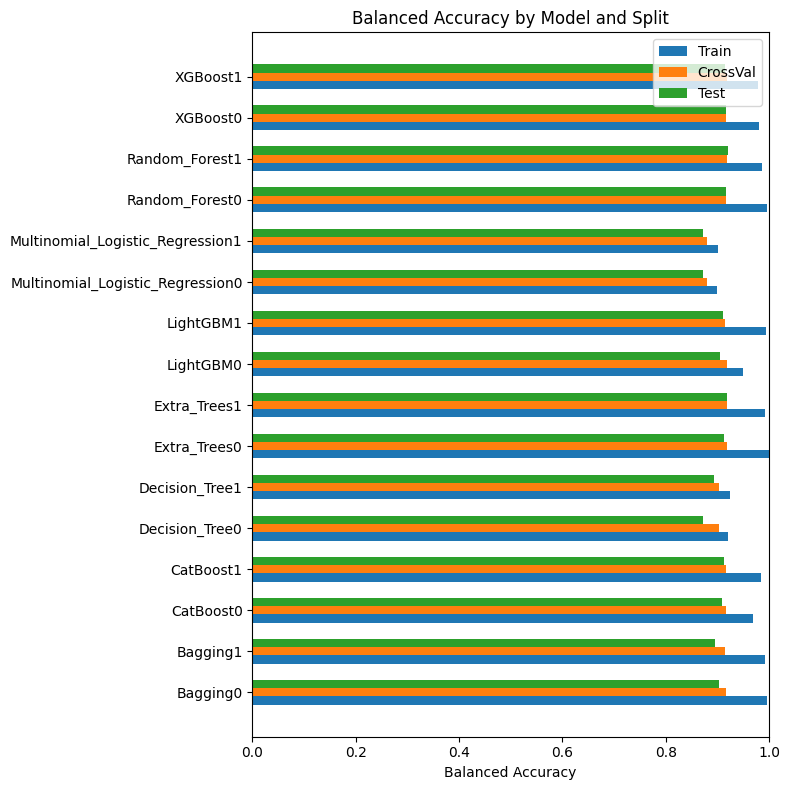
\includegraphics[width=0.65\textwidth]{images/1_Evaluation.png}
	\label{fig:Evaluation with CDRSB, LDELTOTAL, and mPACCdigit}
	\caption{Evaluation of Balanced Accuracies with CDRSB, LDELTOTAL, and mPACCdigit (from folder results/all\_models/1)}
\end{figure}

\begin{figure}[H]
	\centering
	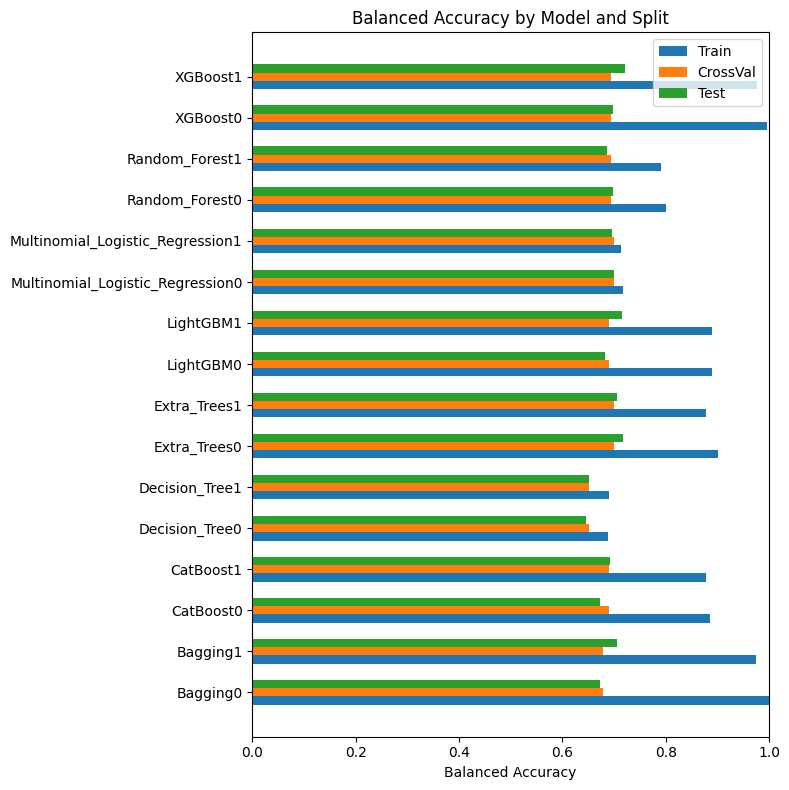
\includegraphics[width=0.65\textwidth]{images/2_Evaluation.png}
	\label{fig:Evaluation without CDRSB, LDELTOTAL, and mPACCdigit}
	\caption{Evaluation of Balanced Accuracies without CDRSB, LDELTOTAL, and mPACCdigit (from folder results/all\_models/2)}
\end{figure}

\newpage

\begin{figure}[H]
	\centering
	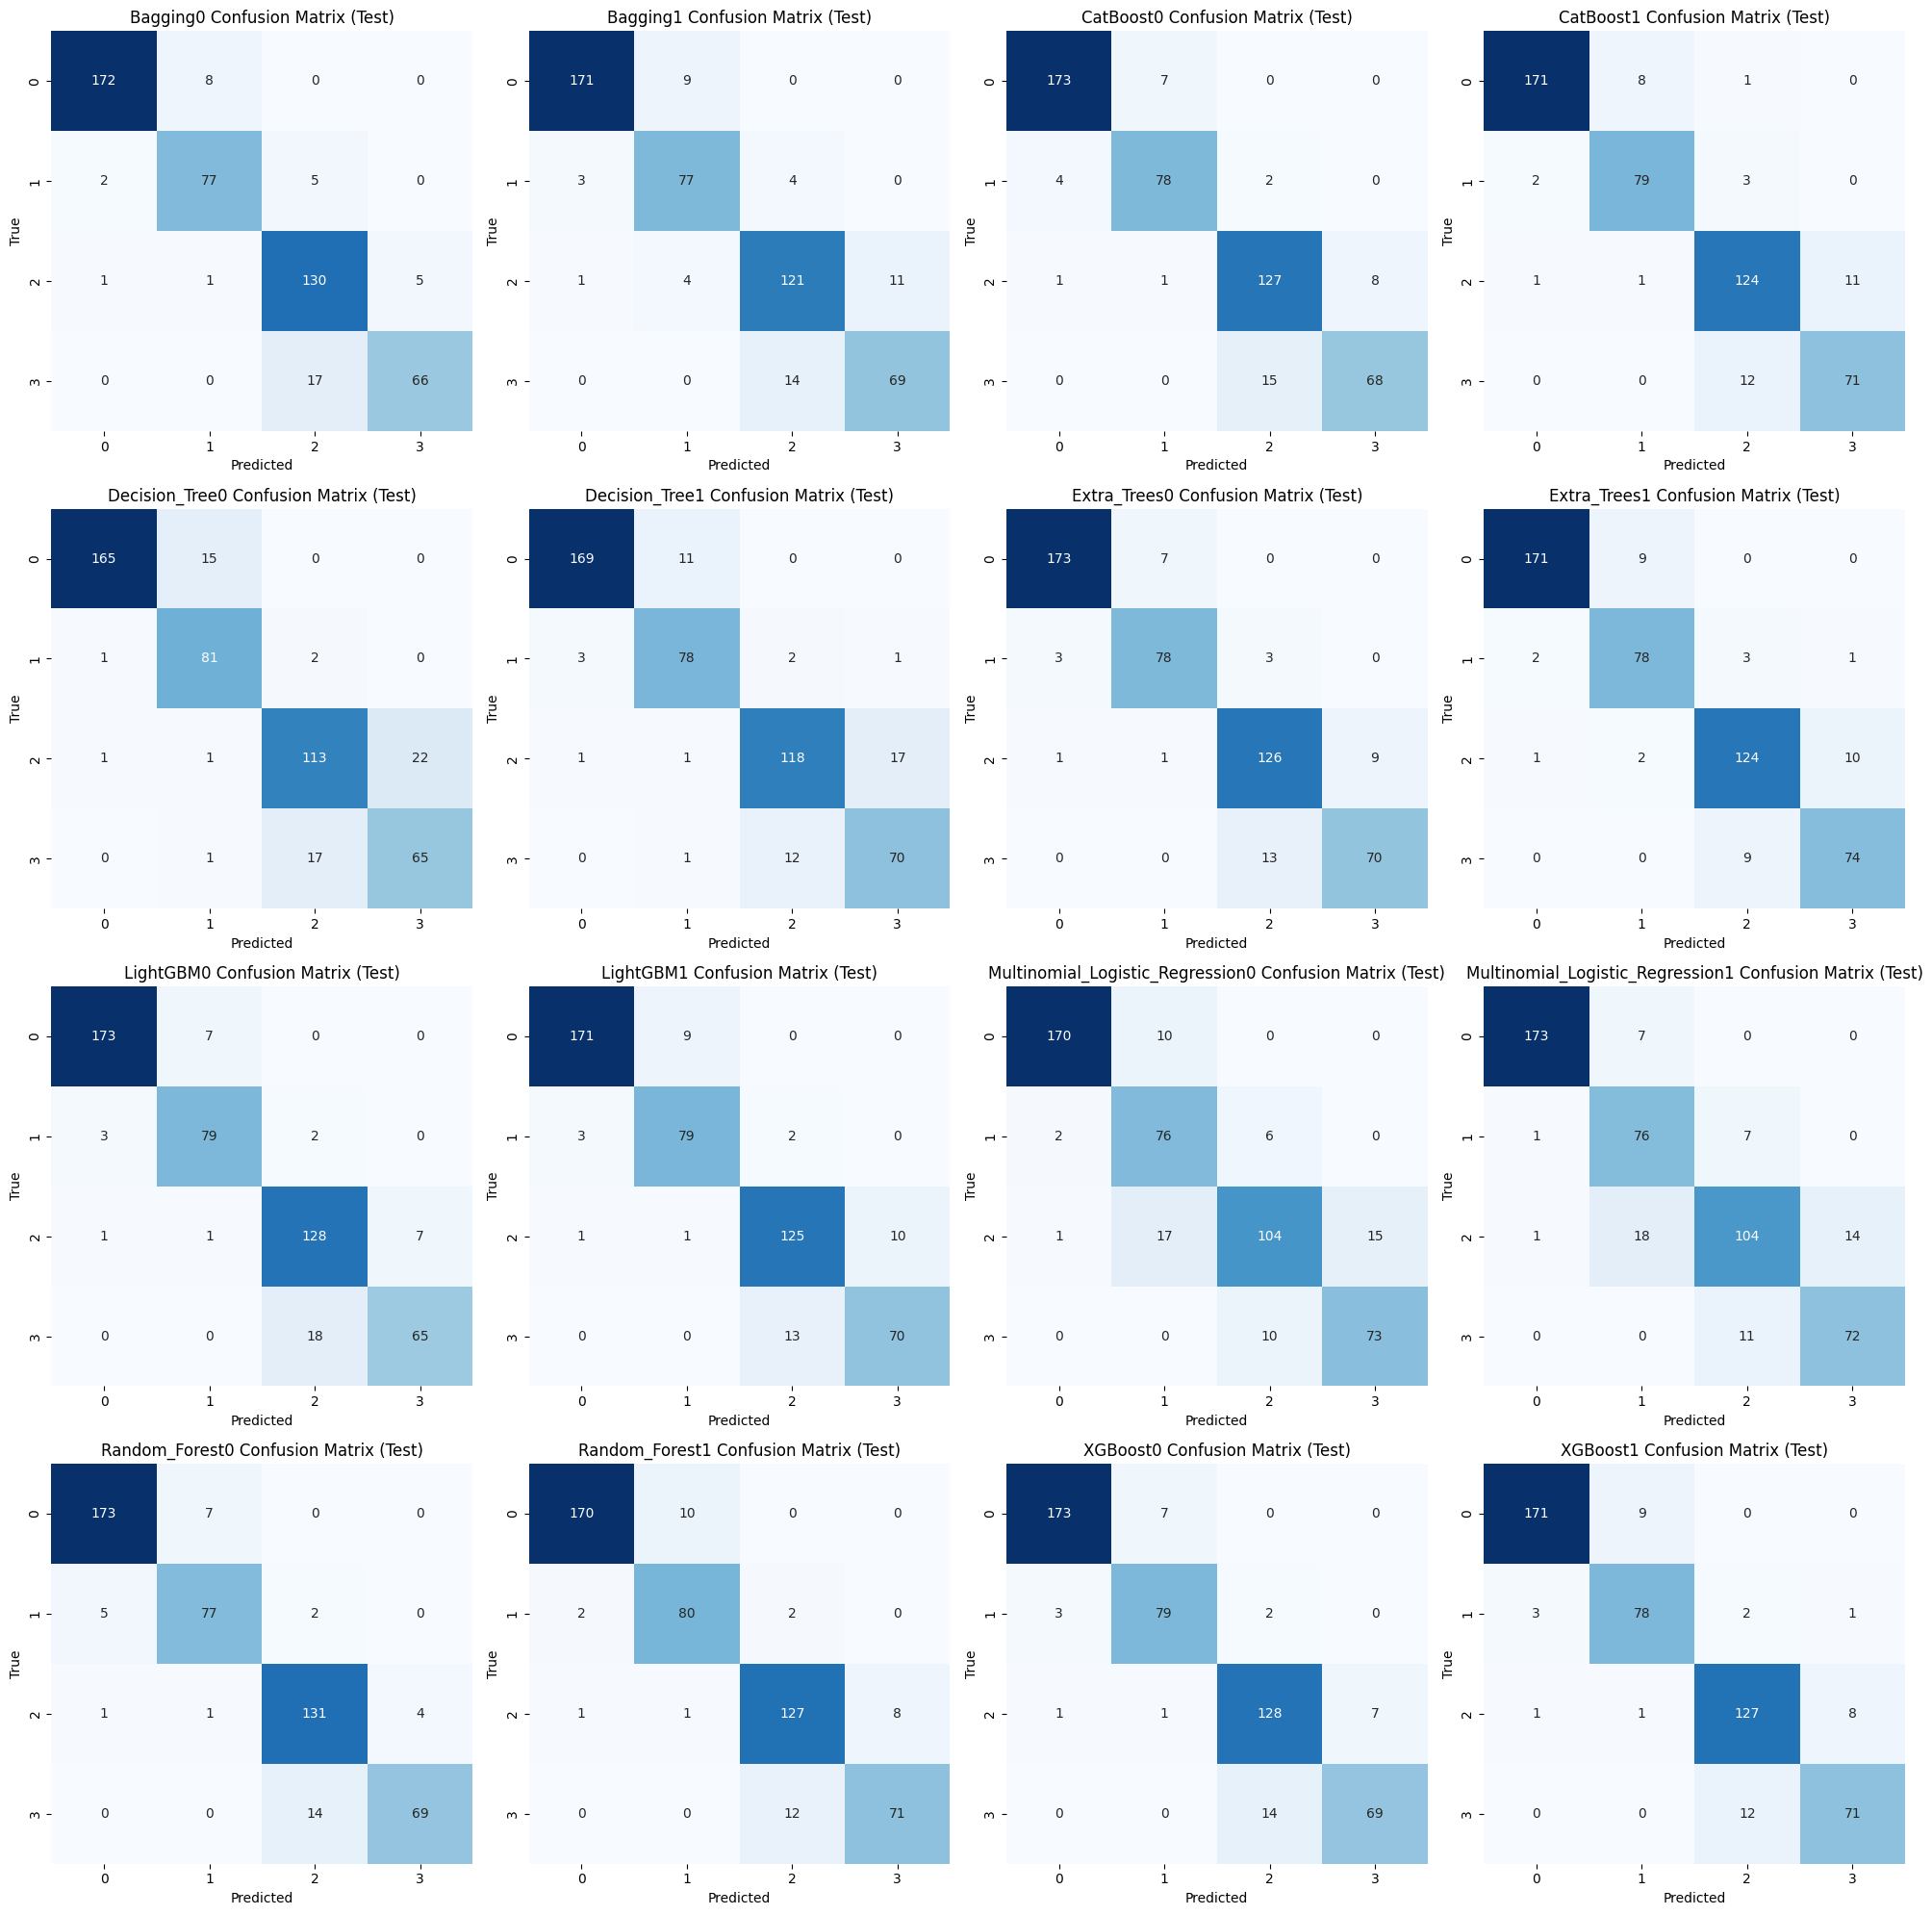
\includegraphics[width=1\textwidth]{images/1_Confusion_Matrix.png}
	\label{fig:Confusion Matrix with CDRSB, LDELTOTAL, and mPACCdigit}
	\caption{Confusion Matrix with CDRSB, LDELTOTAL, and mPACCdigit (from folder results/all\_models/1)}
\end{figure} 

\newpage

\begin{figure}[H]
	\centering
	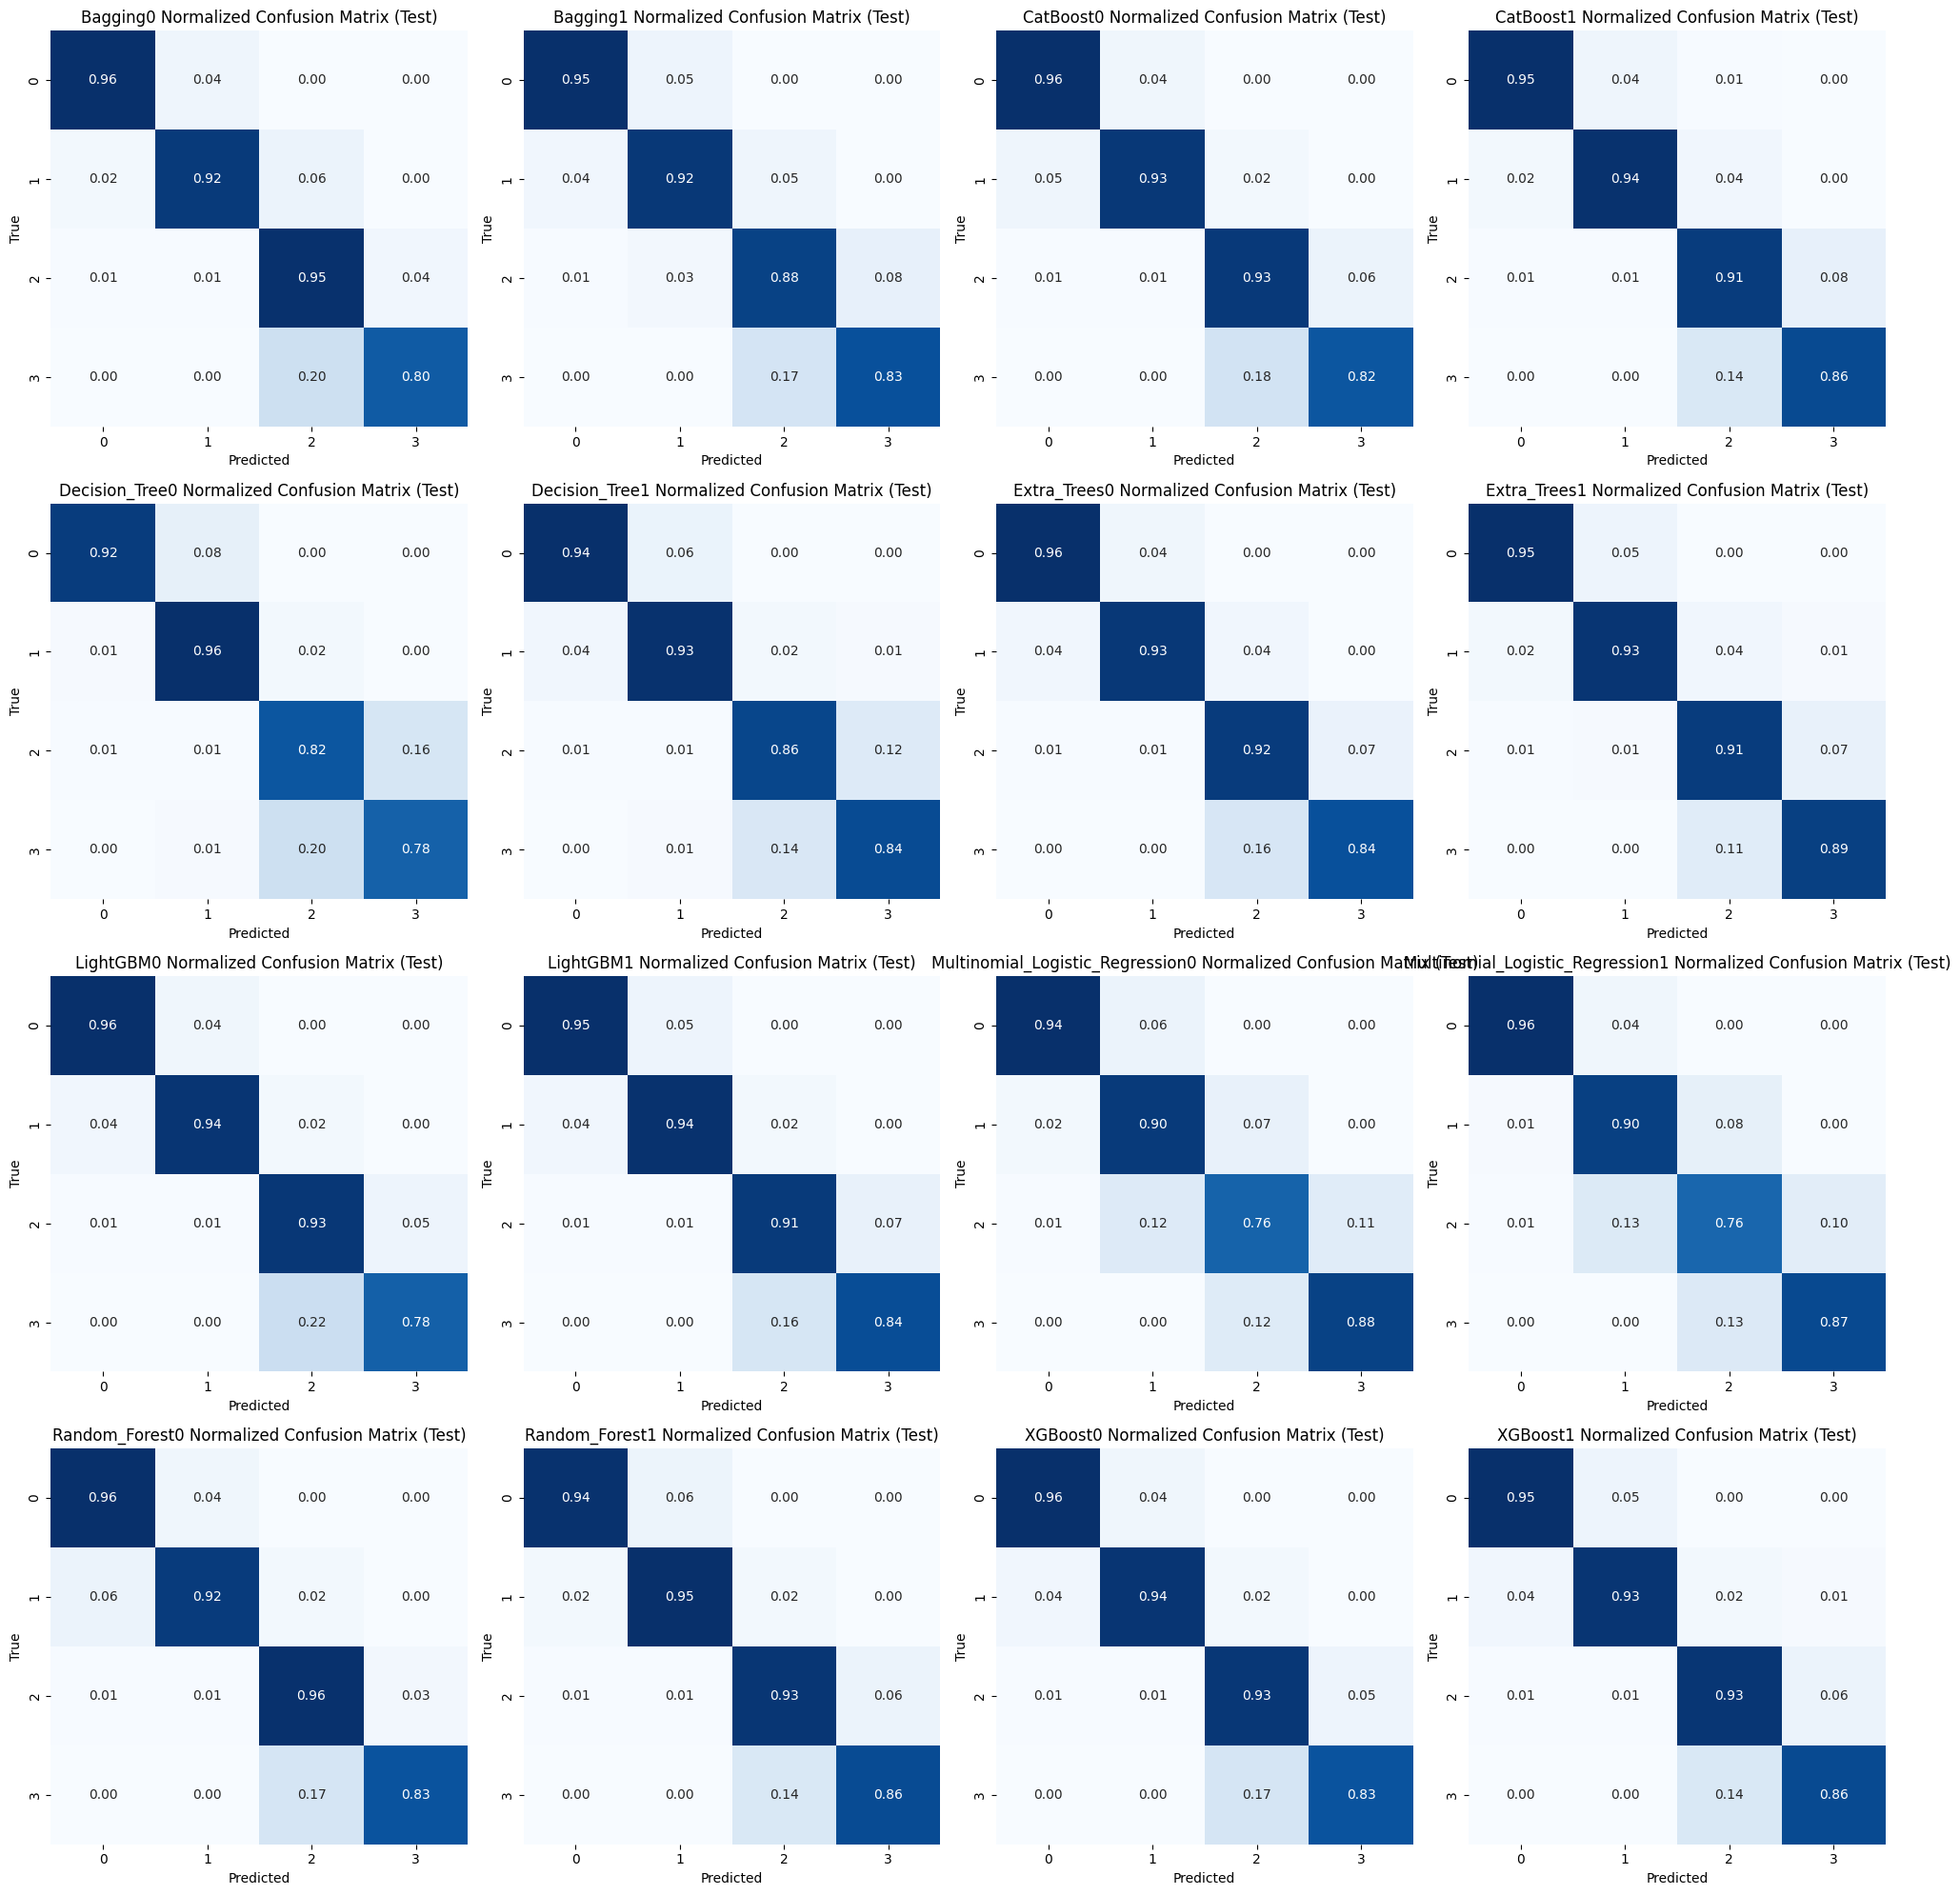
\includegraphics[width=1\textwidth]{images/1_Confusion_Matrix_Normalized.png}
	\label{fig:Normalized Confusion Matrix with CDRSB, LDELTOTAL, and mPACCdigit}
	\caption{Normalized Confusion Matrix with CDRSB, LDELTOTAL, and mPACCdigit (from folder results/all\_models/1)}
\end{figure}

\newpage

\begin{figure}[H]
	\centering
	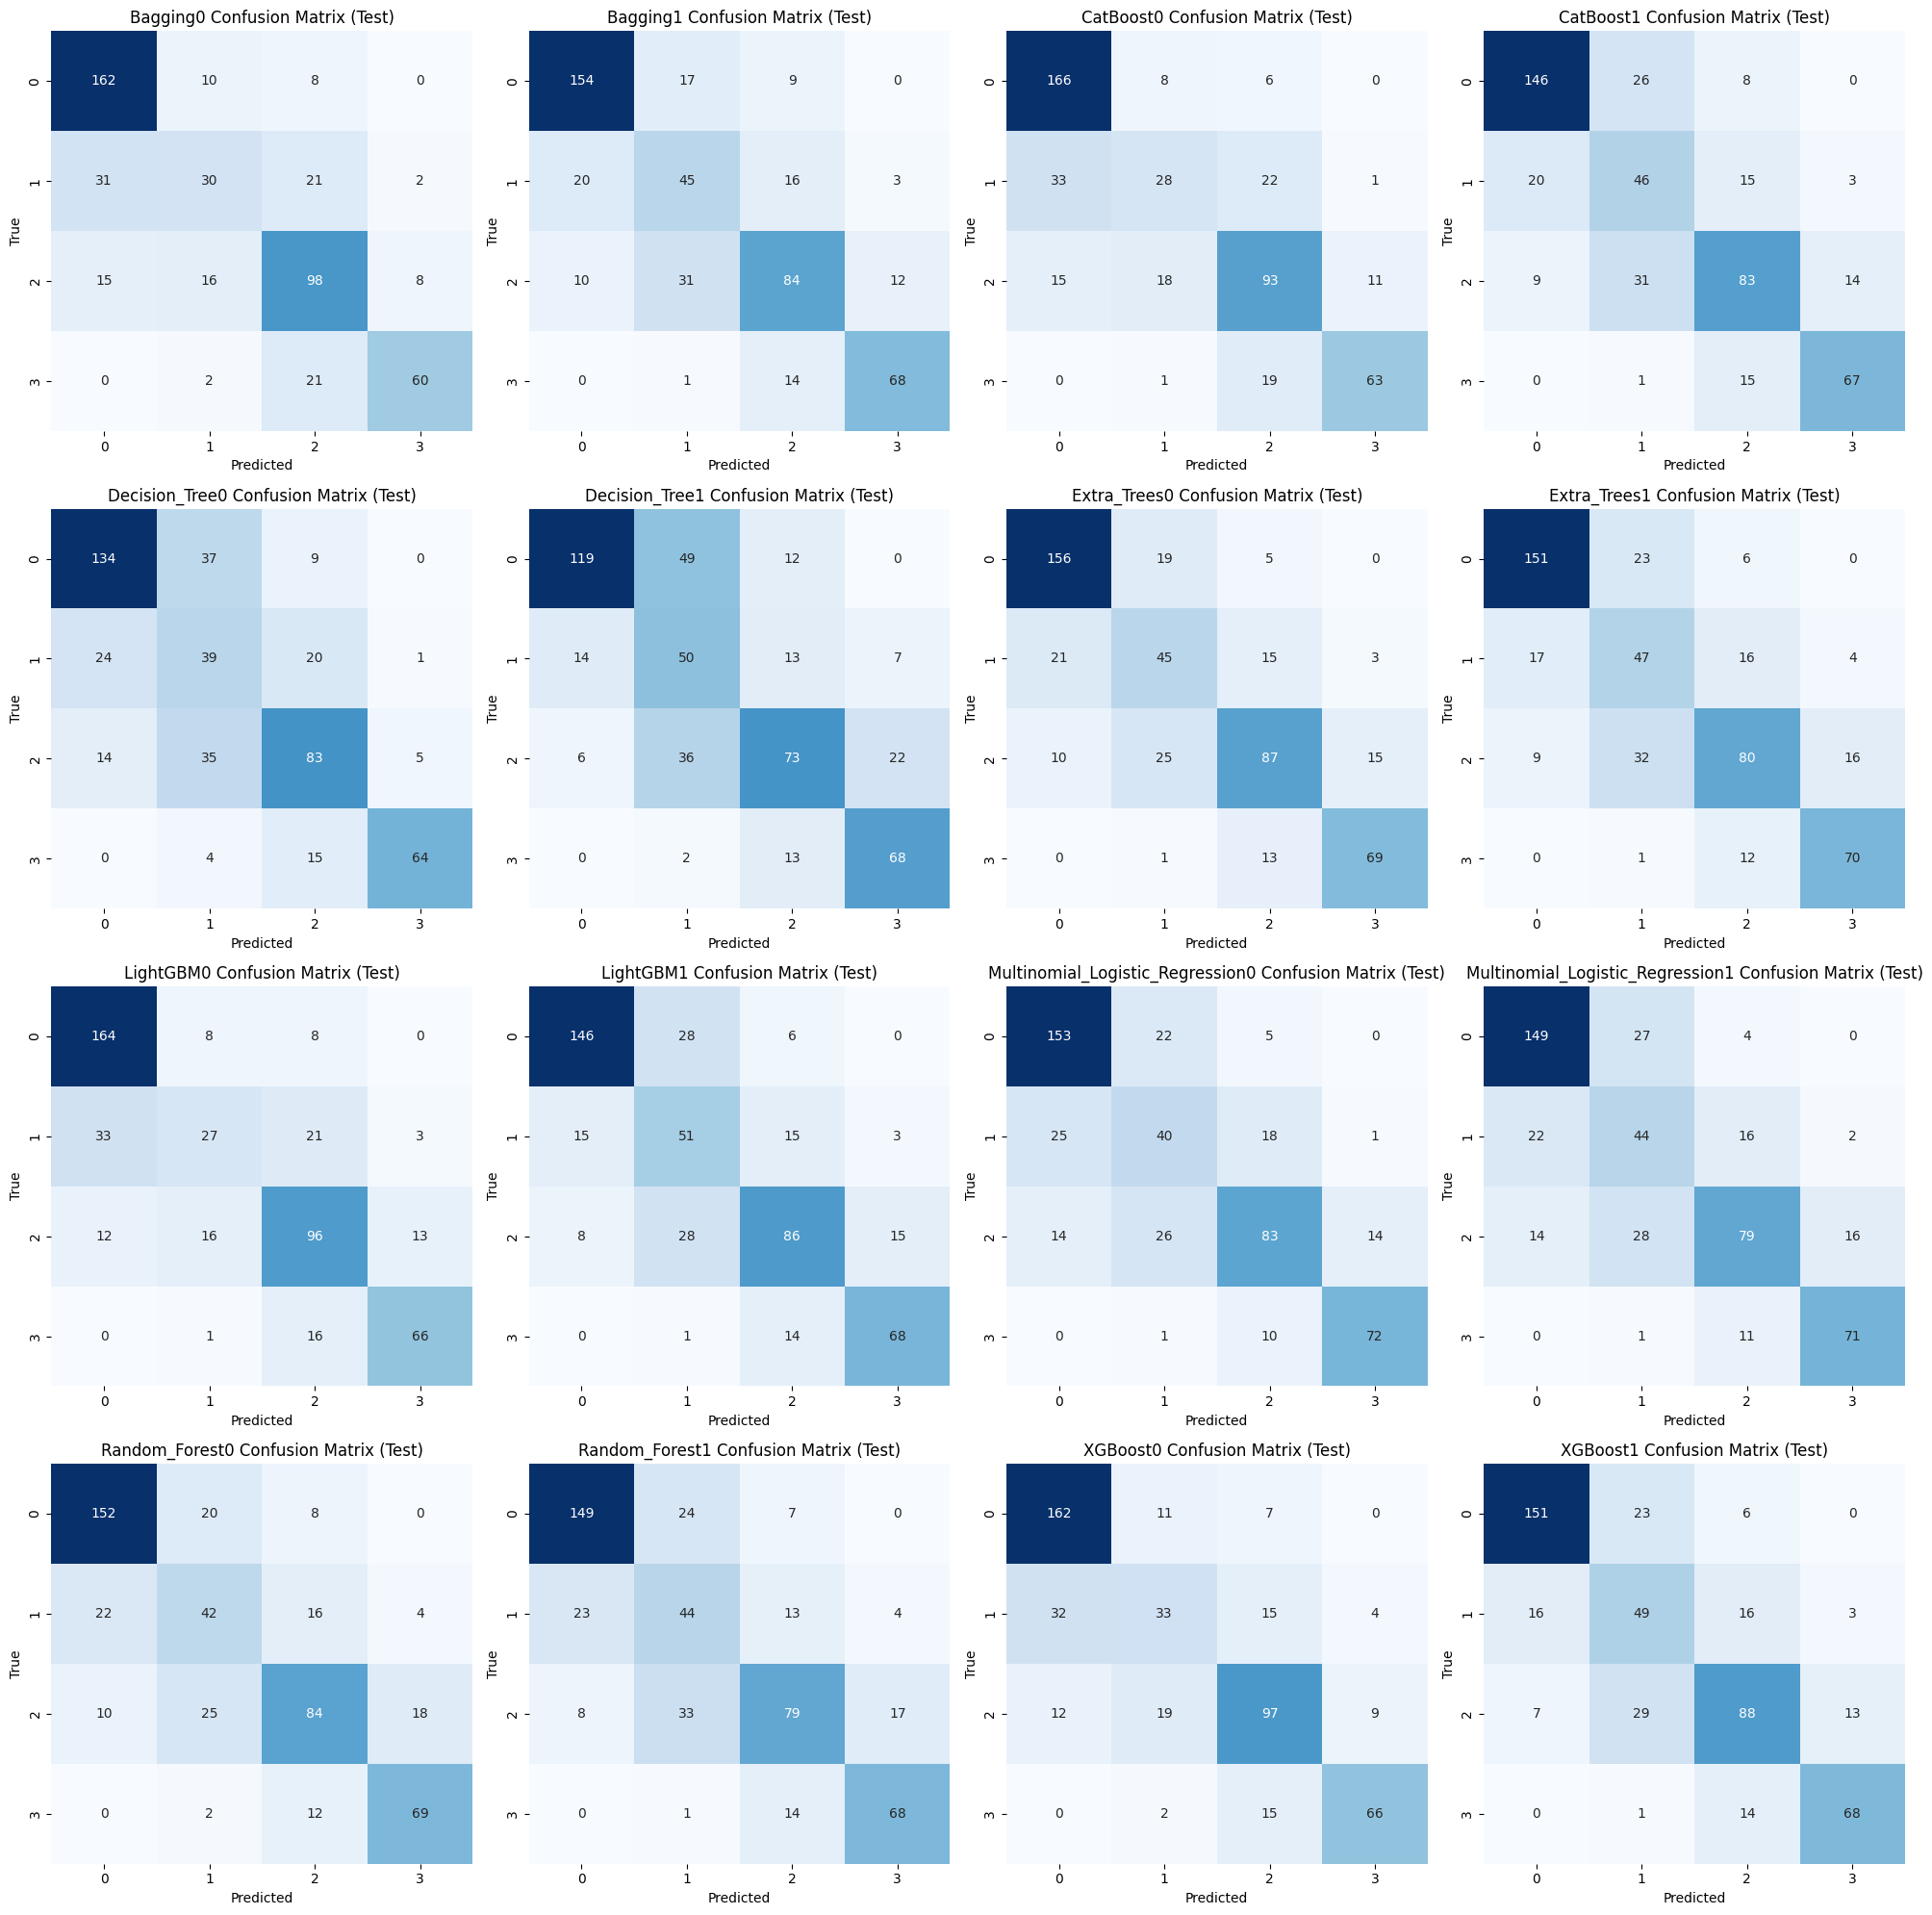
\includegraphics[width=1\textwidth]{images/2_Confusion_Matrix.png}
	\label{fig:Confusion Matrix without CDRSB, LDELTOTAL, and mPACCdigit}
	\caption{Confusion Matrix without CDRSB, LDELTOTAL, and mPACCdigit (from folder results/all\_models/2)}
\end{figure} 

\newpage

\begin{figure}[H]
	\centering
	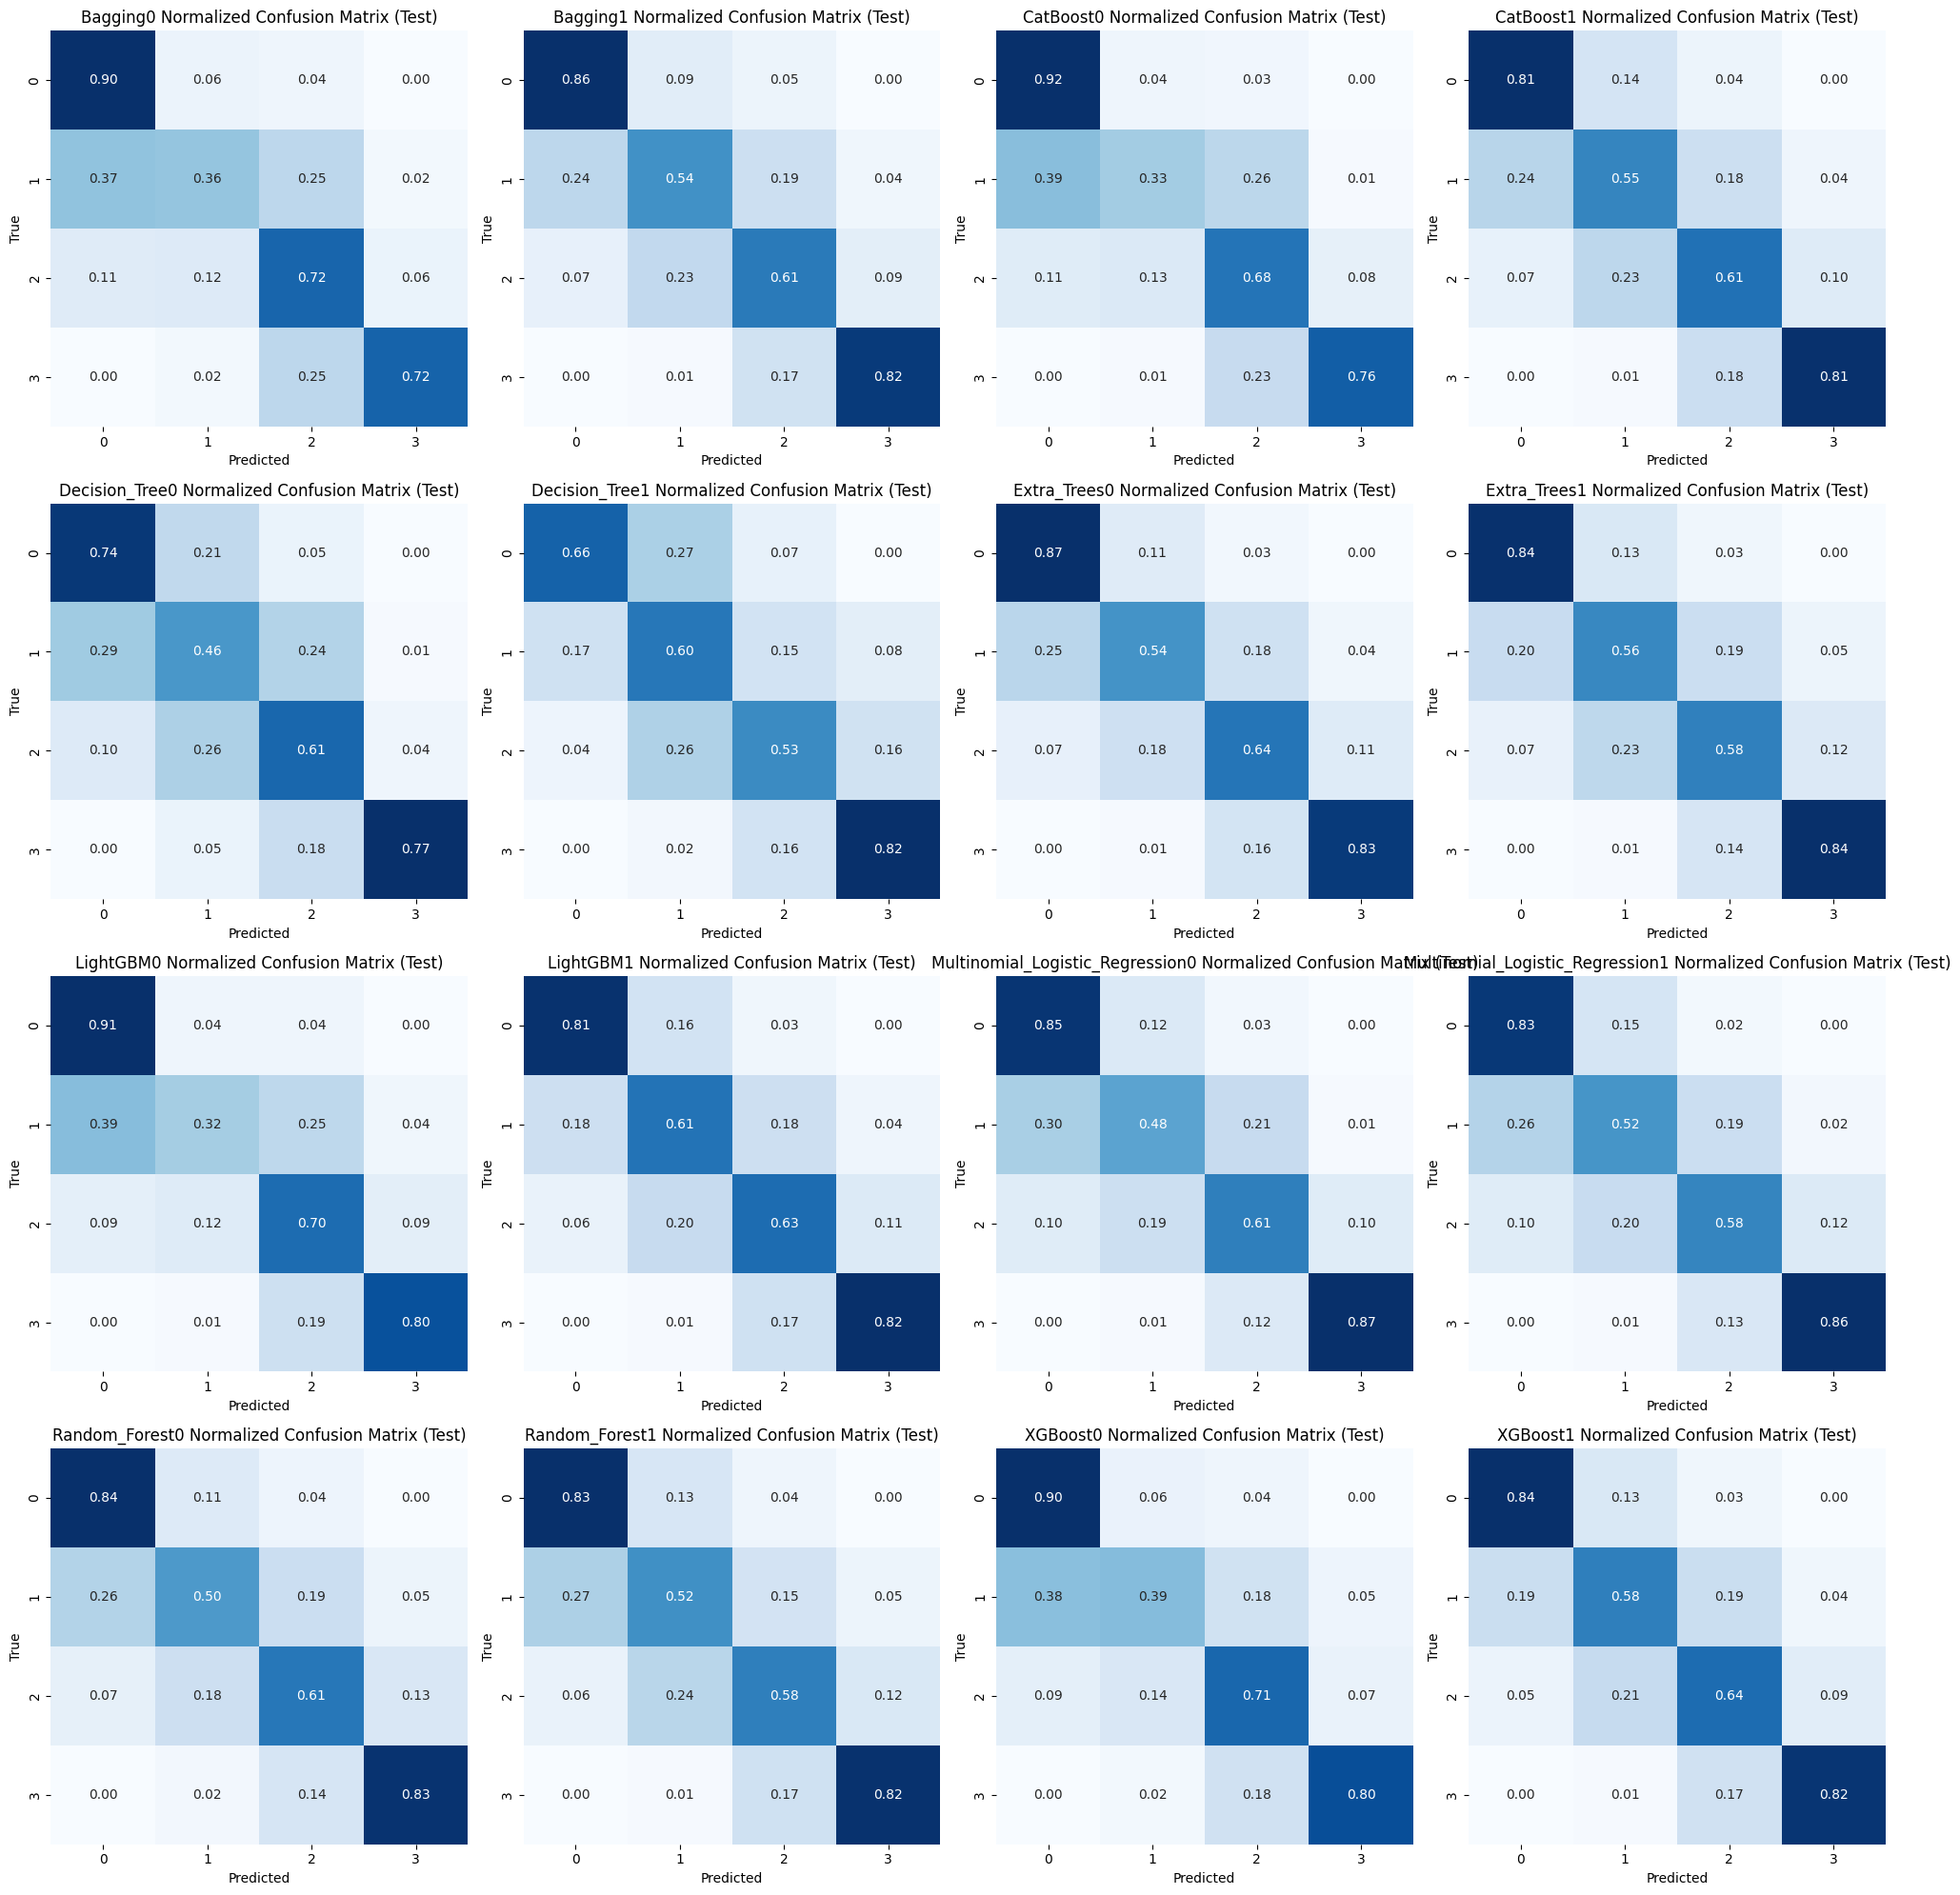
\includegraphics[width=1\textwidth]{images/2_Confusion_Matrix_Normalized.png}
	\label{fig:Normalized Confusion Matrix without CDRSB, LDELTOTAL, and mPACCdigit}
	\caption{Normalized Confusion Matrix without CDRSB, LDELTOTAL, and mPACCdigit (from folder results/all\_models/2)}
\end{figure}

\newpage

\textit{M\_L\_R is for Multinomial\_Logistic\_Regression.}

\vspace{4mm}

\textbf{With CDRSB, LDELTOTAL, and mPACCdigit (from folder results/all\_models/1)}

\begin{tabularx}{\textwidth}{l *{7}{>{\centering\arraybackslash}X}}
	\toprule
	Model & Accuracy & Balanced Accuracy & Precision (weighted) & Recall (weighted) & F1 Score (weighted) & F1 Score (macro) & ROC AUC (macro) \\
	\midrule
	Random\_Forest1 & 0.9256 & 0.9198 & 0.9271 & 0.9256 & 0.9258 & 0.9169 & 0.9865 \\
	Extra\_Trees1 & 0.9236 & 0.9188 & 0.9250 & 0.9236 & 0.9240 & 0.9143 & 0.9862 \\
	XGBoost0 & 0.9277 & 0.9168 & 0.9284 & 0.9277 & 0.9275 & 0.9180 & 0.9876 \\
	Random\_Forest0 & 0.9298 & 0.9163 & 0.9310 & 0.9298 & 0.9294 & 0.9205 & 0.9839 \\
	XGBoost1 & 0.9236 & 0.9153 & 0.9244 & 0.9236 & 0.9237 & 0.9138 & 0.9868 \\
	Extra\_Trees0 & 0.9236 & 0.9132 & 0.9240 & 0.9236 & 0.9236 & 0.9136 & 0.9884 \\
	CatBoost1 & 0.9194 & 0.9128 & 0.9205 & 0.9194 & 0.9197 & 0.9102 & 0.9875 \\
	LightGBM1 & 0.9194 & 0.9116 & 0.9202 & 0.9194 & 0.9195 & 0.9095 & 0.9871 \\
	CatBoost0 & 0.9215 & 0.9090 & 0.9219 & 0.9215 & 0.9212 & 0.9108 & 0.9887 \\
	LightGBM0 & 0.9194 & 0.9048 & 0.9207 & 0.9194 & 0.9189 & 0.9075 & 0.9843 \\
	Bagging0 & 0.9194 & 0.9041 & 0.9224 & 0.9194 & 0.9192 & 0.9079 & 0.9844 \\
	Bagging1 & 0.9050 & 0.8953 & 0.9062 & 0.9050 & 0.9053 & 0.8930 & 0.9835 \\
	Decision\_Tree1 & 0.8988 & 0.8930 & 0.9015 & 0.8988 & 0.8995 & 0.8862 & 0.9803 \\
	M\_L\_R1 & 0.8781 & 0.8731 & 0.8831 & 0.8781 & 0.8785 & 0.8629 & 0.9806 \\
	Decision\_Tree0 & 0.8760 & 0.8722 & 0.8813 & 0.8760 & 0.8771 & 0.8615 & 0.9746 \\
	M\_L\_R0 & 0.8740 & 0.8720 & 0.8811 & 0.8740 & 0.8748 & 0.8598 & 0.9815 \\
	\bottomrule
\end{tabularx}

\vspace{4mm}

\textbf{Without CDRSB, LDELTOTAL, and mPACCdigit (from folder results/all\_models/2)}

\begin{tabularx}{\textwidth}{l *{7}{>{\centering\arraybackslash}X}}
	\toprule
	Model & Accuracy & Balanced Accuracy & Precision (weighted) & Recall (weighted) & F1 Score (weighted) & F1 Score (macro) & ROC AUC (macro) \\
	\midrule
	XGBoost1 & 0.7355 & 0.7210 & 0.7458 & 0.7355 & 0.7392 & 0.7172 & 0.9071 \\
	Extra\_Trees0 & 0.7376 & 0.7172 & 0.7383 & 0.7376 & 0.7368 & 0.7140 & 0.9093 \\
	LightGBM1 & 0.7252 & 0.7163 & 0.7400 & 0.7252 & 0.7301 & 0.7098 & 0.9081 \\
	Extra\_Trees1 & 0.7190 & 0.7064 & 0.7285 & 0.7190 & 0.7211 & 0.6988 & 0.9068 \\
	Bagging1 & 0.7252 & 0.7059 & 0.7282 & 0.7252 & 0.7258 & 0.7043 & 0.9038 \\
	M\_L\_R0 & 0.7190 & 0.6999 & 0.7188 & 0.7190 & 0.7172 & 0.6970 & 0.9071 \\
	XGBoost0 & 0.7397 & 0.6990 & 0.7287 & 0.7397 & 0.7314 & 0.7033 & 0.9126 \\
	Random\_Forest0 & 0.7169 & 0.6972 & 0.7173 & 0.7169 & 0.7159 & 0.6919 & 0.9053 \\
	M\_L\_R1 & 0.7087 & 0.6959 & 0.7160 & 0.7087 & 0.7093 & 0.6900 & 0.9037 \\
	CatBoost1 & 0.7066 & 0.6930 & 0.7180 & 0.7066 & 0.7106 & 0.6894 & 0.9092 \\
	Random\_Forest1 & 0.7025 & 0.6869 & 0.7116 & 0.7025 & 0.7045 & 0.6809 & 0.9040 \\
	LightGBM0 & 0.7293 & 0.6821 & 0.7127 & 0.7293 & 0.7152 & 0.6827 & 0.9123 \\
	Bagging0 & 0.7231 & 0.6738 & 0.7138 & 0.7231 & 0.7131 & 0.6824 & 0.9040 \\
	CatBoost0 & 0.7231 & 0.6734 & 0.7089 & 0.7231 & 0.7101 & 0.6786 & 0.9093 \\
	Decision\_Tree1 & 0.6405 & 0.6521 & 0.6881 & 0.6405 & 0.6522 & 0.6357 & 0.8567 \\
	Decision\_Tree0 & 0.6612 & 0.6464 & 0.6904 & 0.6612 & 0.6726 & 0.6547 & 0.8380 \\
	\bottomrule
\end{tabularx}

\newpage
\begin{multicols}{2}
\subsection{Final Decision}
For the dataset containing the three highly predictive cognitive scores (CDRSB, LDELTOTAL, mPACCdigit), \textbf{\textit{Random\_Forest1}} (\textbf{the RF trained with the hybrid sampling strategy}) was chosen as the main model, and \textbf{\textit{Decision\_Tree1}} (\textbf{the version with sampling}) was chosen as the reference XAI model. This choice is motivated by very high test metrics (balanced accuracy, F1, ROC-AUC) that show the best sensitive tradeoff between classes.

\textbf{Model1.pkl and XAIModel1.pkl are respectively Random\_Forest1 and Decision\_Tree1.}

\vspace{4mm}

For the dataset where those three cognitive scores were removed, the model that maintained the best performance was \textbf{\textit{XGBoost1}} (XGBoost with hybrid sampling), and, again, \textbf{\textit{Decision\_Tree1}} was chosen as the XAIModel (the version built on the dataset without the three scores). This selection also comes from comparing the metrics on the test set. 

\textbf{Model2.pkl and XAIModel2.pkl are respectively XGBoost1 and Decision\_Tree1.} 


